\section{Metodología}\label{sec-metología}

La metodología del presente estudio se centra un análisis de contenido
del discurso multimodal \cite{jewitt2017,norris2019} de una selección de
\emph{booktoks} en español para identificar los nuevos usos e
interacciones frente a la cámara para hablar de vídeos.

Pero previamente, se debe explicar cómo se ha llegado a la selección de
vídeos final. A partir de los planteamientos de \emph{Netnografía} de
\textcite{kozinets2021}, se ha realizado una primera selección de 500 booktoks
para conocer las etiquetas más usadas y las características generales de
estos vídeos. En febrero de 2020, poco antes del inicio del
confinamiento provocado por la covid-19 se creó un perfil específico
para la investigación. El acceso inicial estuvo mediado por las
sugerencias de la herramienta. Cabe recordar que esta propone dos
opciones: ``Siguiendo'' (\emph{Following}), donde aparecen los vídeos de
los perfiles a los que uno sigue; y ``Para ti'' (\emph{For} \emph{You})
con vídeos nuevos según los intereses que la herramienta considera que
uno tiene, ofreciendo dos vías de acceso a nuevos vídeos. Además, se
precisa que los resultados ofrecidos dependen de lo que considere el
algoritmo asignado a cada cuenta y que estos datos pueden estar mediados
por los datos compartidos en cada dispositivo móvil. El algoritmo de
TikTok puede modificar los resultados de cualquier búsqueda \cite{siles2022,jones2023}. Deben considerarse
los sesgos informacionales en este tipo de estudio en plataformas
propiciados por la ausencia de neutralidad de las plataformas \cite{vandijck2013,sumpter2018,hepp2020} en la presentación de resultados
o la conexión con otras redes sociales o el historial de navegación
asociado a un usuario \cite{fisher2019,fisher2022}.

En el uso inicial de la plataforma se trabajó específicamente para
conseguir que el algoritmo se centrase en contenidos relacionados con la
lectura y los libros. Para esto se realizaron búsquedas rutinarias con
estos términos: ``book'', ``booktok'', ``lectura'', ``libros'' y
``literatura''. En sucesivas búsquedas se comprobó que no siempre salían
los mismos resultados respecto a vídeos con más reproducciones. A partir
de aquí, se seguían y se identificaban con ``me gusta'' (\emph{like}, un
símbolo de corazón que se marca en rojo) a los vídeos de esta temática.
Aunque siguen apareciendo vídeos de otros contenidos según otros
intereses del investigador y de los datos compartidos de su dispositivo
móvil, se consiguió que más del 50 \% de los vídeos estuvieran
relacionados con estos contenidos. En enero de 2024, este perfil sigue a
más de 7000 cuentas, de los cuáles más de 6000 (más del 80 \%) están
relacionados con nuestra investigación. Posteriormente, la herramienta
incluyó junto a ``me gusta'' la opción de marcar como ``favoritos''
(\emph{favorites}, un símbolo de etiqueta, que se marca en amarillo) a
los vídeos para generar colecciones específicas.

A partir de los planteamientos del citado Kozinets se definen unos
criterios de búsqueda y selección \cite{turpogenebra2008}. Se revisan
otras investigaciones sobre TikTok desde el ámbito educativo para
conocer distintos procedimientos para la selección y clasificación de
los vídeos \cite{tejedorcalvo2022,yélamosguerra2022,caldeiro2023}.

Se establece como pregunta de investigación de caracterización de los
booktoks como nuevos epitextos virtuales para la promoción de la
lectura. Se acota la investigación a TikTok, aunque algunos vídeos
puedan replicarse en otras plataformas como Instagram o sean creados
para Youtube. Se considera por lo tanto que esta plataforma virtual es
un nuevo espacio de especialización en la promoción digital de lectura,
porque además presenta un altísimo tráfico, con millones de vídeos y
usuarios. Aunque la selección de vídeos se ha hecho desde un perfil
concreto y con la influencia del algoritmo de la plataforma, los
\emph{booktoks} están en abierto y ofrece mucha información detallada
tanto de los vídeos como de los usuarios.

Una vez seleccionados los 500 vídeos, se han analizado de forma
individual por los investigadores, para posteriormente poner en común
las características de cada vídeo. En esta ocasión no se tiene en cuenta
en la interacción y audiencia de los vídeos, encontrando alguno con
muchos visionados frente a otros menos conocidos. Los criterios
principales han sido las distintas estrategias multimodales para
presentar la información e intentar señalar las nuevas dinámicas que
ofrece la red. En el presente análisis se ha descartado el análisis de
las interacciones y comentarios de los espectadores, datos fundamentales
que pueden incluirse en posteriores investigaciones. Por último, se han
contrastado las categorías establecidas con usuarios de la plataforma
interesados en la promoción virtual de la literatura.

En dicha cuenta se han destacado 500 vídeos relacionados con esta
categoría en una lista específica. Posteriormente, se concretan los
requisitos: 1. Que sean perfiles activos; 2. Que hayan surgido por
sugerencia del algoritmo en la sección ``Para ti''; 3. Que el contenido
pueda etiquetarse claramente bajo el concepto de \#booktok; 4. Que el
perfil que realiza el vídeo tenga un mínimo de participación e
interacción en la plataforma. Sobre este listado se concretaron las
variables descriptivas \cite{braun2006} y los motivos de exclusión.
Los vídeos tenían que estar en español o creados por perfiles
hispanohablantes, centrados en el ámbito de la lectura y se excluyeron
distintos vídeos (-201) por reiteración de perfiles o dinámicas,
quedando el corpus final en 299 vídeos. Se realiza otro análisis
posterior de manera individual por los investigadores autores, para
señalar los vídeos más significativos. Se señalan 30 perfiles y 30
vídeos más destacados, según las siguientes variables \cite{desantis2000}: V1 audiencia, seguidores y visionados; V2 Uso de
etiquetas; V3 características del vídeo; y V4 análisis multimodal
\cite{kress2001}. La lista final de 10 vídeos se revisa de
acuerdo a las distintas dinámicas identificadas (10 tipos recogidos en
\Cref{tab-02}). La V4 se aplicó solamente a 10 vídeos como aproximación
central de este estudio.

\begin{table}[htpb]
\centering
\begin{threeparttable}
\caption{Proceso para la selección de vídeos.}
\label{tab-01}
\begin{tabular}{p{0.47\textwidth}p{0.47\textwidth}}
\toprule
Perfil individual & Sigue a 7000 cuentas \\
Lista pública de \#Booktok & Se incluyen en la lista 500 vídeos \\
Se aplican requisitos y criterios de exclusión & Se destacan 299
\emph{booktoks}, diferenciando sus características. \\
Se realiza análisis de variables & Se señalan 30 perfiles y 30 vídeos
(no recogidos en esta publicación) \\
Se identifican 10 tipologías distintas & Se identifican como
dinámicas \\
\multicolumn{2}{l}{Se realiza el análisis multimodal recogido en los resultados} \\
\bottomrule
\end{tabular}
\source{Elaboración propia.}
\end{threeparttable}
\end{table}


Desde febrero de 2023 se creó la Colección ``Booktok''
(\url{https://www.tiktok.com/@joseroviracollado/collection/Booktok-7193946691401796357})
que ha servido como instrumento principal para nuestra investigación,
que en enero de 2024 cuenta con 500 vídeos relacionados con esta
categoría. La mayoría de los vídeos están en español o creados por
perfiles hispanohablantes, aunque se pueden encontrar también algunos en
inglés u otras lenguas para identificar o comparar dinámicas, todos
están centrados en el ámbito de la lectura y en la selección se
excluyeron varios vídeos por reiteración de perfiles o dinámicas. Aunque
aparecen algunos vídeos en inglés u otras lenguas, los vídeos de nuestro
análisis están en español, o alguna de sus etiquetas o el perfil creador
es hispanohablante. A partir de esta colección se identificaron
distintas dinámicas de interacción en \emph{booktok} \cite{roviracollado2022}, entendiendo como dinámicas distintos usos de los
\emph{booktok} para hablar de libros. Se ha limitado la muestra a 10
tipos de dinámicas distintas para concretar nuestro análisis multimodal.

Los vídeos citados son accesibles en abierto en marzo de 2024 sin
necesidad de darse de alta en la plataforma, por lo que se respeta el
nivel de privacidad que han seleccionado tanto las personas creadoras de
los mismos como los usuarios que participan en los comentarios.
Solamente se comentan los perfiles personales de personas que se pueden
considerar microcelebridades por la audiencia recibida. Una vez
analizados sus diferentes contenidos se han identificado diez dinámicas
distintas \Cref{tab-02} para la promoción de contenido literario en la
plataforma a los que se les ha aplicado un análisis del discurso
multimodal \cite{kress2001}. Se aplica el análisis a estos
diez vídeos diferentes para señalar los distintos usos que se realizan
en la categoría de \emph{booktok}. Se busca ofrecer distintas
posibilidades dentro del análisis multimodal para destacar la amplitud
de vídeos que se recogen bajo esta categoría.


\begin{table}[htbp]
\centering
\begin{threeparttable}
\caption{Selección de vídeos y descripción de las diferentes dinámicas.}\label{tab-02}
\begin{tabular}{p{0.47\textwidth}p{0.47\textwidth}}
\toprule
Dinámica & Hipervículo \\
\midrule
1. ¿Qué estás leyendo ahora?\newline
What are you reading? & \url{https://www.tiktok.com/@claudiacp_books/video/7230137545923792155} \\
2. Fiesta de Seguidores\newline
Readers follow party &
\url{https://www.tiktok.com/@laslecturasdeloli/video/6972178596152511749} \\
3. Bibliotecas &
\url{https://www.tiktok.com/@bibliotecaugena/video/6971466004585057542} \\
4. Tipos de Booktoker &
\url{https://www.tiktok.com/@pandi.book/video/7199333140748438790}\\
5. Promoción lectora &
\url{https://www.tiktok.com/@iriayselene/video/7211269180484750598} \\
6. Editoras &
\url{https://www.tiktok.com/@vreditorasya/video/7223140662022114565} \\
7. Bookinfluencer &
\url{https://www.tiktok.com/@patriciafedz/video/7222221715819072774} \\
8. Día del libro &
\url{https://www.tiktok.com/@javierruescas/video/7224553867566910747}\\
9. Videopoemas &
\url{https://www.tiktok.com/@marinalcuadrado/video/7173687644935703814} \\
10. Así dijo\ldots{} &
\url{https://www.tiktok.com/@solo.palabrqs/video/7190817595401030918} \\
\bottomrule
\end{tabular}
\source{Elaboración propia.}
\end{threeparttable}
\end{table}

Existen otras muchas dinámicas que provienen del \emph{booktuber} como
los \emph{Unboxing} (abrir un paquete), \emph{Wishlist} (lista de
deseos) o \emph{Wrap} \emph{Up} (resumen de los libros leídos en un
periodo), que adaptan las dinámicas previas \cite{soto2015} a la
ubicuidad de los móviles. También los \emph{booktrailer} o bibliotráiler
\cite{tabernero2018} se difunden ya a través del móvil, por lo que
sería una categoría heredada dentro de los \emph{booktoks} y no algo
distinto a los \emph{booktubers} \cite{roviracollado2017}. En esta
investigación no se realiza un análisis descriptivo del éxito de los
distintos \emph{booktoks}, por lo que no se prioriza en señalar el
número de visualizaciones, ``me gusta'' o comentarios.

Se comienza con la identificación de estas diez dinámicas recurrentes y
se aplica un análisis semiótico social a partir del estudio de las
relaciones interpersonales que ofrecen las diferentes personas creadoras
de contenido (como personajes representados) en estas dinámicas
atendiendo a la \emph{focalización} (contacto visual y perspectiva),
\emph{distancia} \emph{social} (alejamiento o proximidad del plano) y
\emph{actitud} (diferenciando la angulación vertical y horizontal). Las
diferentes opciones aparecen en la \Cref{fig-image1} siguiendo las aportaciones
de \textcite{canamares2021} y \textcite{martínez-carratala}. No se han tenido en cuenta criterios específicos para el
análisis del texto.

\begin{figure}[htbp]
\begin{minipage}{\textwidth}
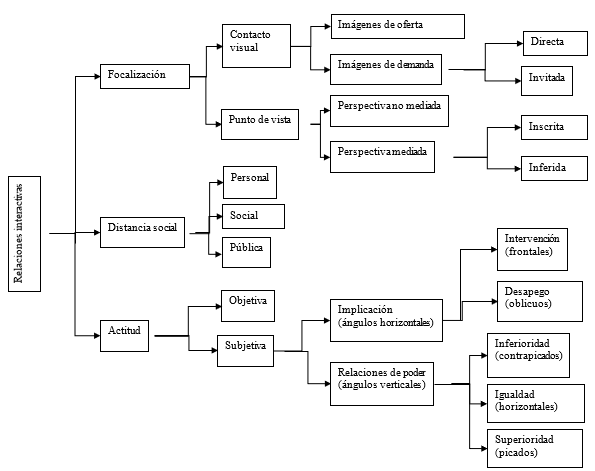
\includegraphics[width=\textwidth]{image1}
\caption{Sistema de relaciones interactivas del discurso multimodal.}
\label{fig-image1}
\source{\textcite[p. 6]{martínez-carratala}}	
\end{minipage}
\end{figure}

El interés de la investigación se centra en las relaciones
interpersonales dada la importancia de las elecciones de las personas
creadoras de contenido en establecer una relación interactiva con su
audiencia con capacidad de influencia en la interpretación y valoración
del contenido representado, siendo los libros muchas veces los
principales protagonistas. En este punto, se describen brevemente los
diferentes sistemas para guiar la presentación de la sección de
resultados y los diferentes grados de implicación que establecen con su
audiencia. En primer lugar, la focalización se articula a partir de dos
posibilidades, como son el \emph{contacto} \emph{visual} y la
\emph{imagen de oferta}. Cuando el contacto es directo demanda una mayor
implicación y empatía a la audiencia frente a la \emph{imagen} \emph{de}
\emph{oferta} donde se es meramente espectadores de los hechos
representados. Respecto al punto de vista, las opciones con mayor
implicación se producen cuando la perspectiva es \emph{mediada} y se
incluye a la audiencia en el campo visual de la persona representada con
dos opciones: \emph{inscrita}, cuando se contempla la situación
representada desde sus espaldas o \emph{inferida,} cuando la audiencia
contempla las acciones desde el mismo campo visual que la persona
creadora del vídeo (punto de vista subjetivo). Igualmente, el sistema de
\emph{distancia} \emph{social} está referido al uso del plano que marca
la proximidad entre la persona creadora y quienes contemplan: de manera
general, una mayor proximidad (el empleo de un primer plano) provoca una
mayor cercanía (personal) que no un plano donde la persona que crea el
vídeo se muestra muy alejada. En una plataforma donde los contenidos son
creados principalmente a través del móvil, este tipo de cercanía a
través del plano es evidentemente más frecuente. Finalmente, el sistema
de \emph{actitud} está referido a la angulación horizontal y vertical,
donde en el plano horizontal delimita la implicación con la audiencia
(frontales, una mayor implicación y oblicuos un mayor dinamismo y
desapego al salir de la imagen) y el vertical las relaciones de poder
(si la audiencia contempla a la persona desde un ángulo picado se
encuentra en superioridad o en inferioridad si se contempla a la persona
representada desde abajo en un ángulo contrapicado).
